
\begin{frame}{\citetitle{Escanner3D_Aleman2022}$^*$  (1)}
\begin{columns}
\begin{column}{0.6\textwidth}
	\begin{itemize}
		\item Muchas de las tareas que tradicionalmente se hacían en una PC ahora han migrado hacia el teléfono inteligente
        \item La digitalización de objetos 3D ha tenido un auge en tiempos recientes
		\item El escaner se obtiene datos de un sensor ultrasónico montado en un motor (escaneo vertical)
		\item Una plataforma giratoria rota el objeto para obtener los datos desde todos los ángulos
	\end{itemize}
\end{column}
\begin{column}{0.4\textwidth}  
\begin{center}
     \begin{tabular}{c}
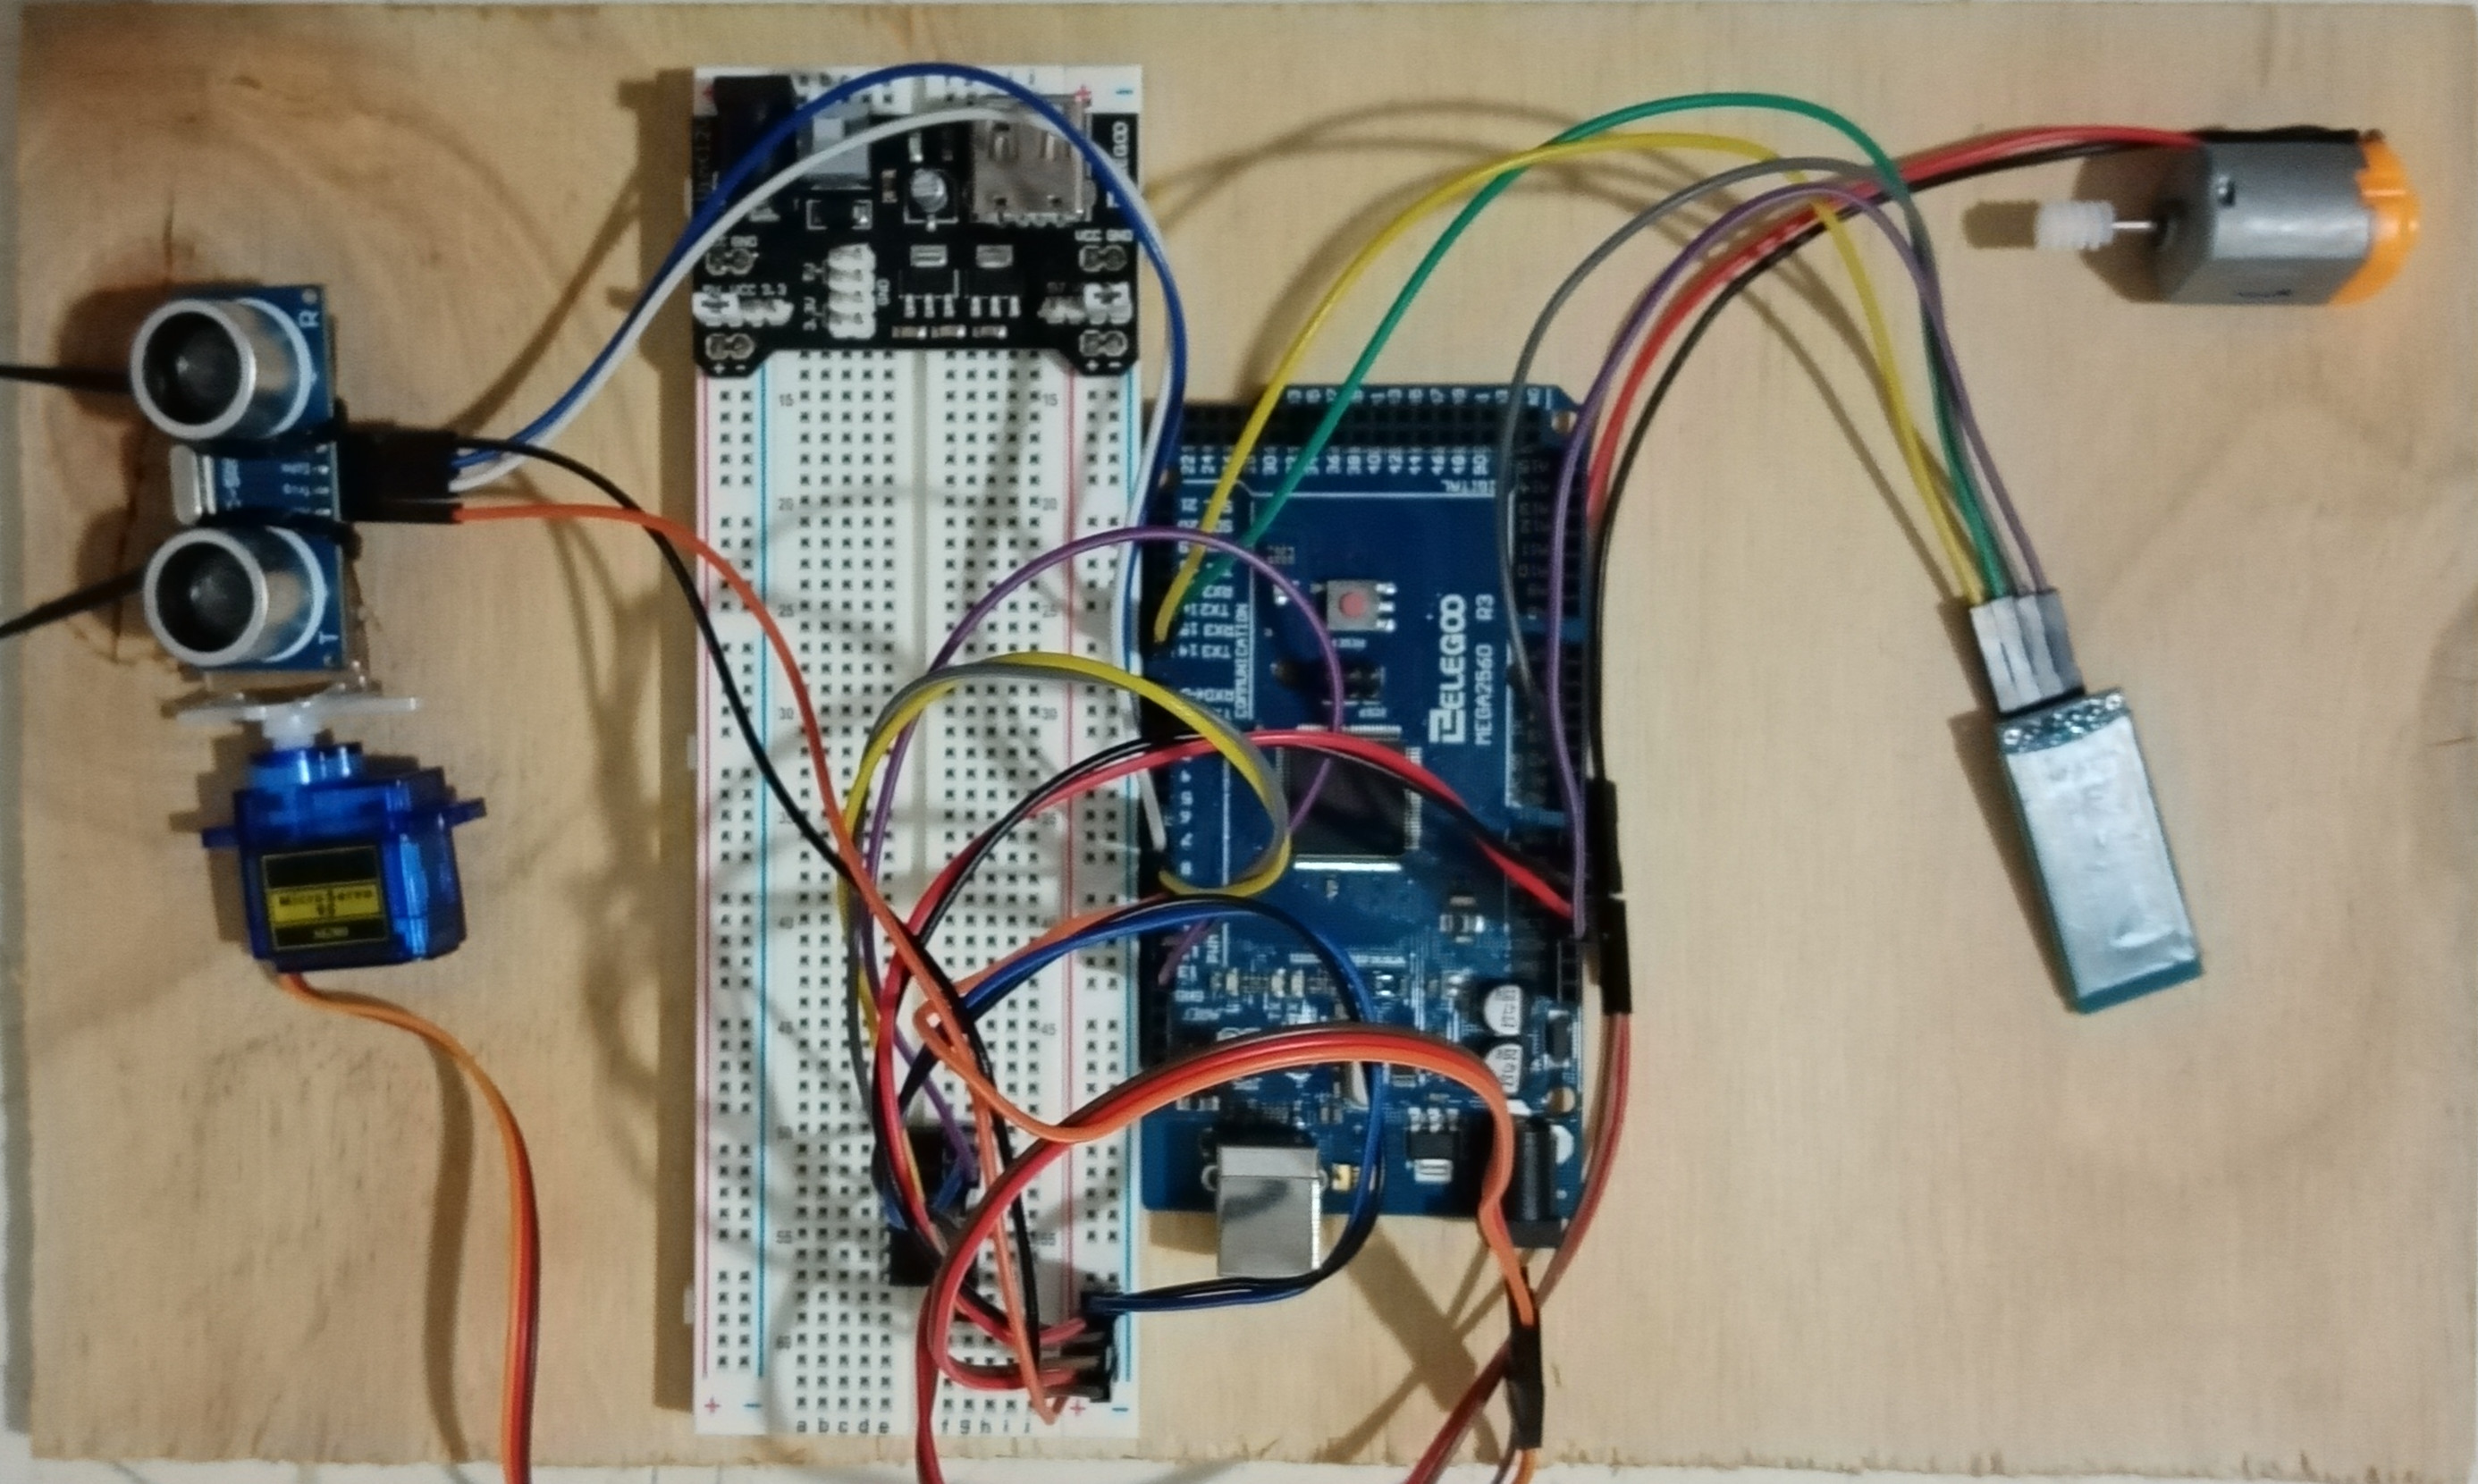
\includegraphics[width=0.68\textwidth]{2022_Scanner3D/figs/Esc1}\\
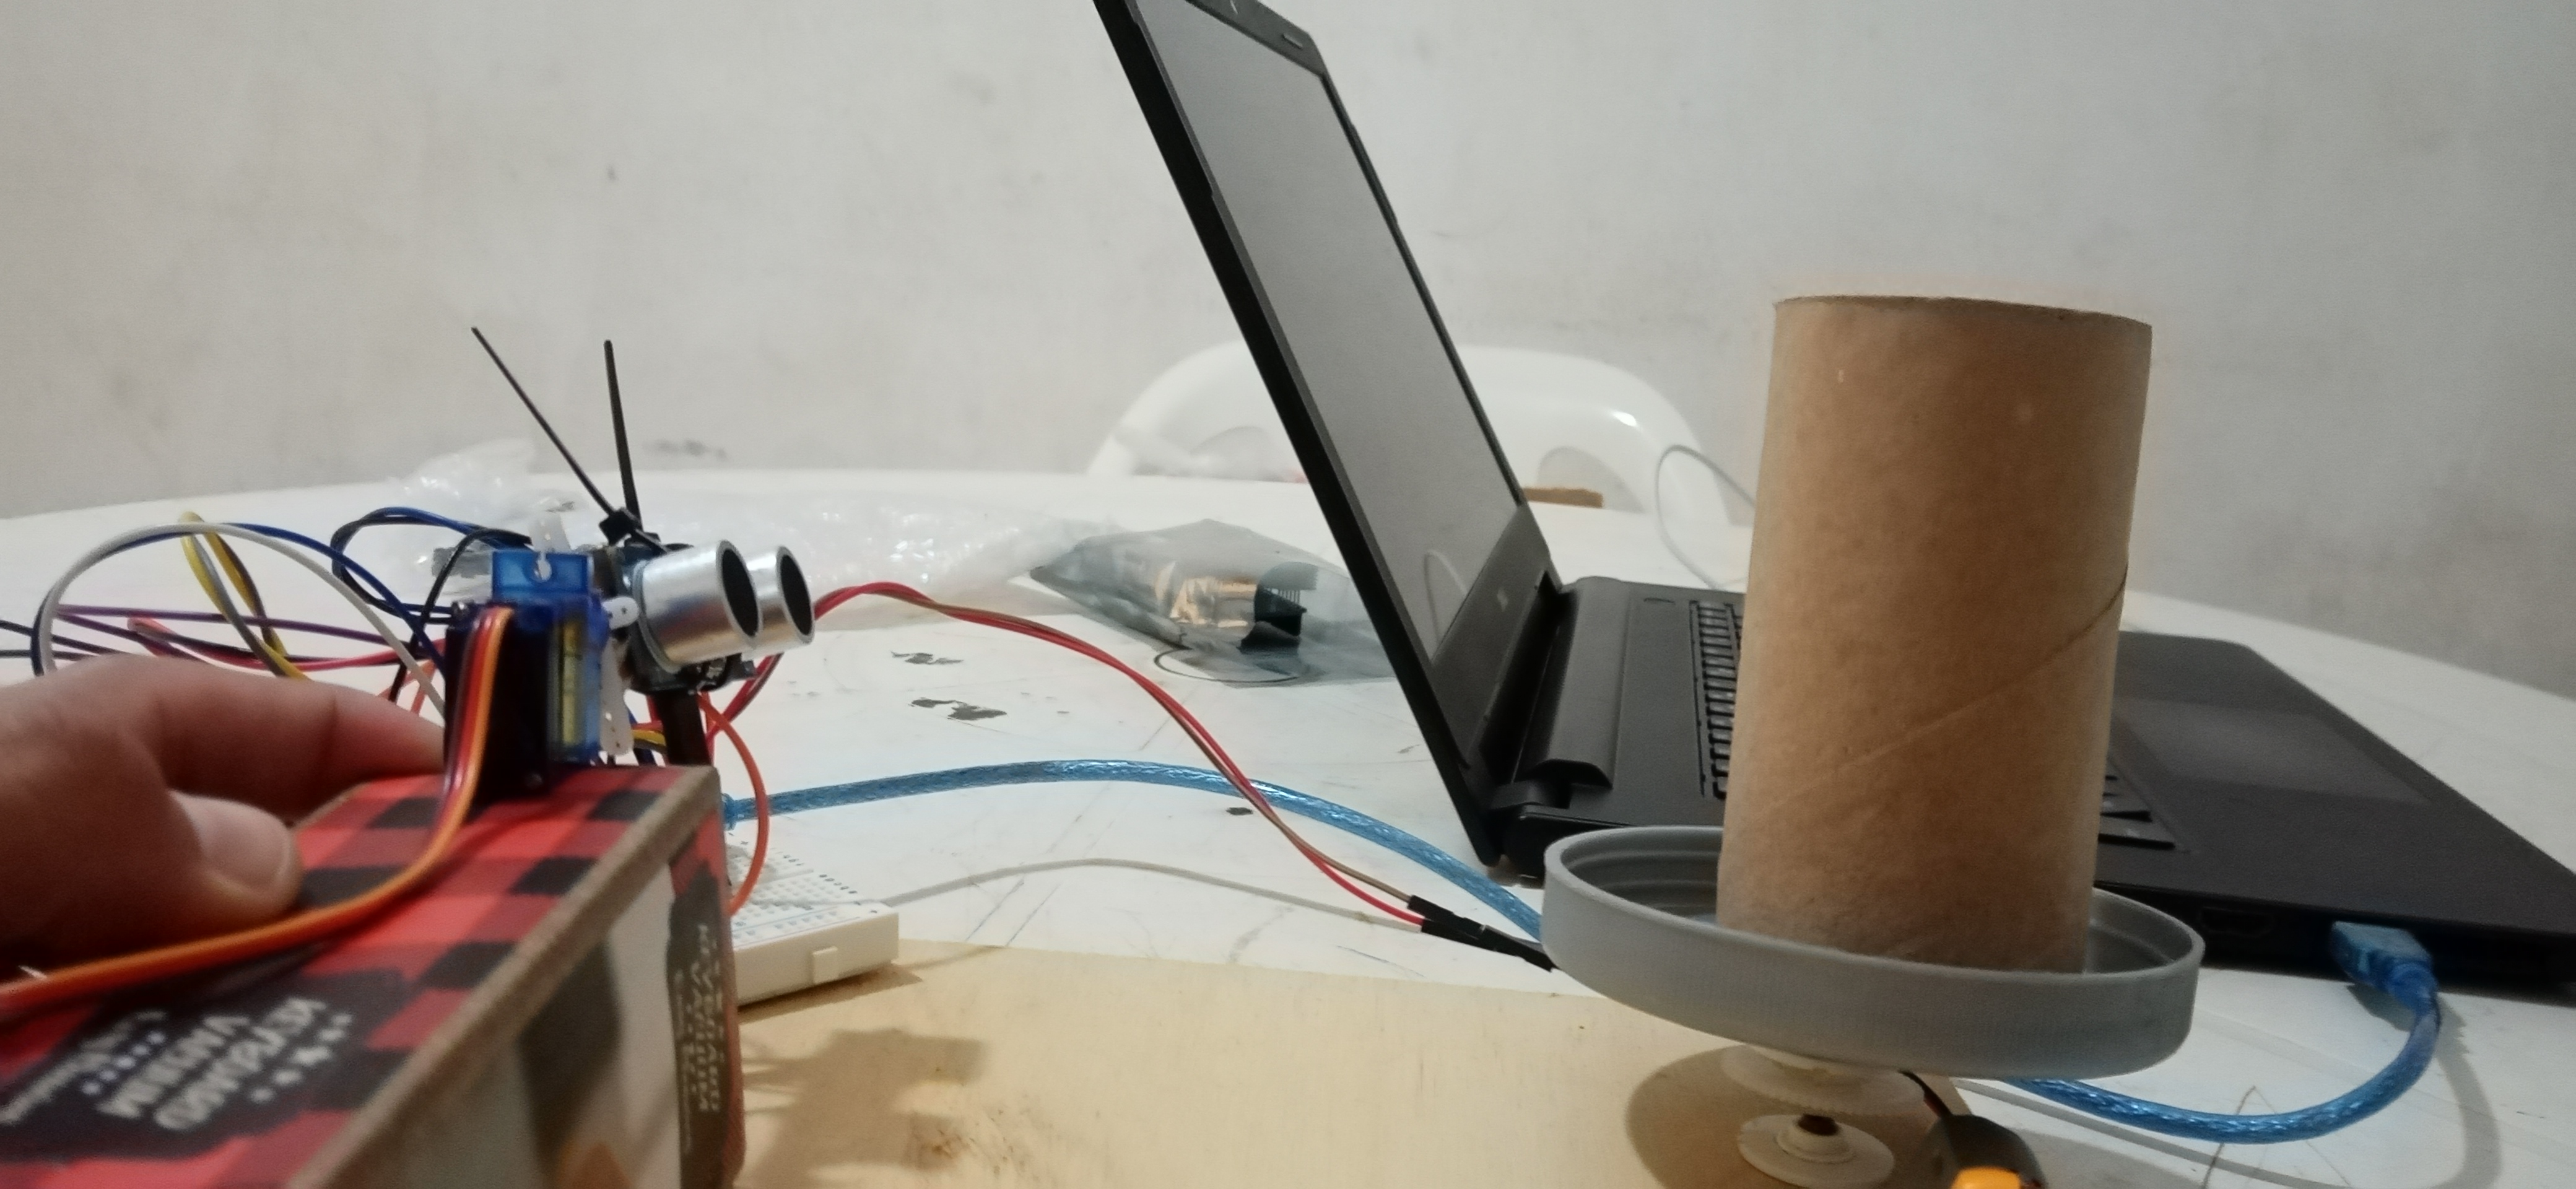
\includegraphics[width=0.68\textwidth]{2022_Scanner3D/figs/Esc2}\\         
      \end{tabular}
\end{center}
\end{column} 
\end{columns} 
\footfullcite*{Escanner3D_Aleman2022}
\end{frame}


\begin{frame}{\citetitle{Escanner3D_Aleman2022} (2)}
	\begin{itemize}
        \item La aplicación visualiza el modelo adquirido y lo almacena en un formato estándar
        \item Se propone una App para un escaner 3D ``casero'' mediante comunicación Bluetooth
	\end{itemize}
\begin{center}
 \begin{tabular}{cccc}
    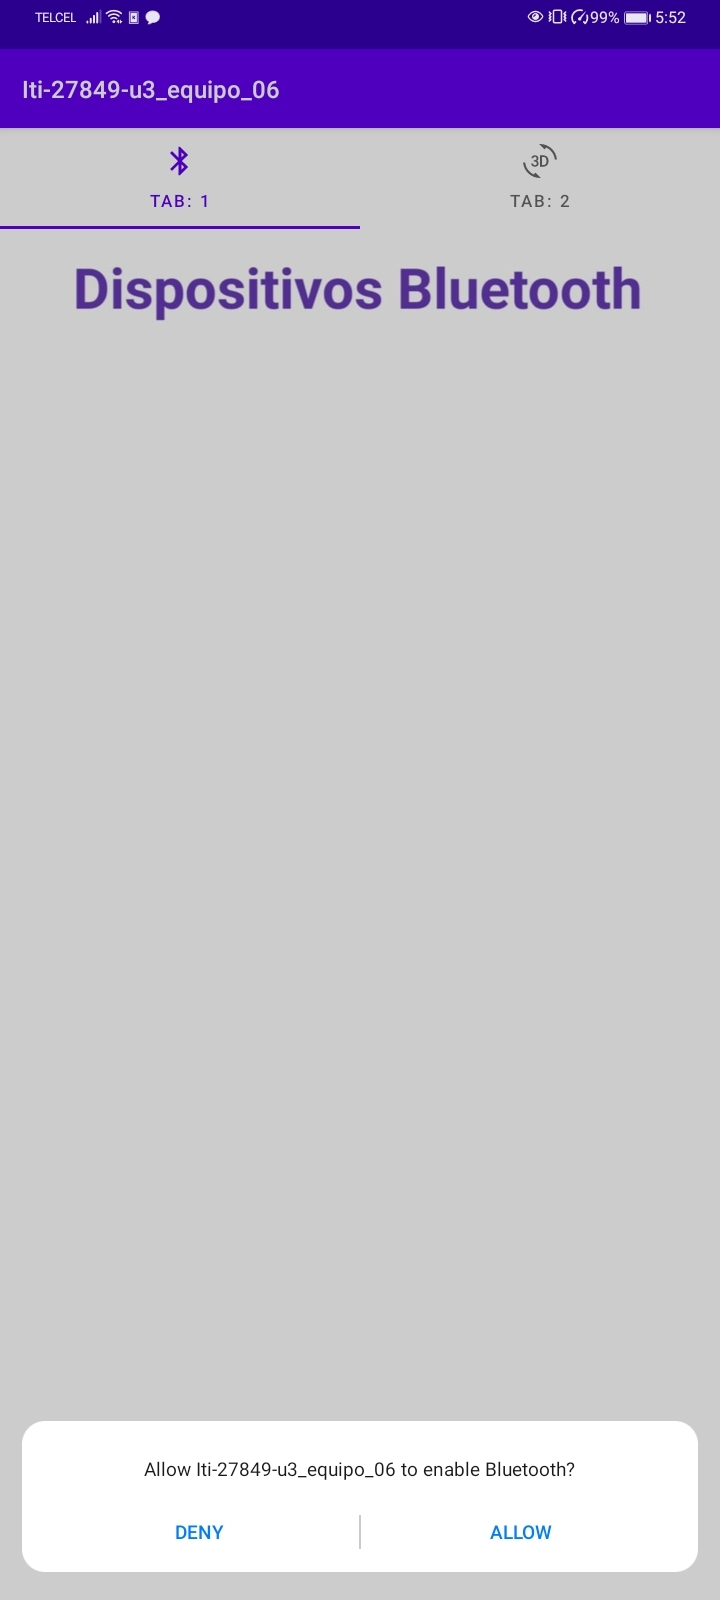
\includegraphics[width=0.14\textwidth]{2022_Scanner3D/figs/Ap1}
    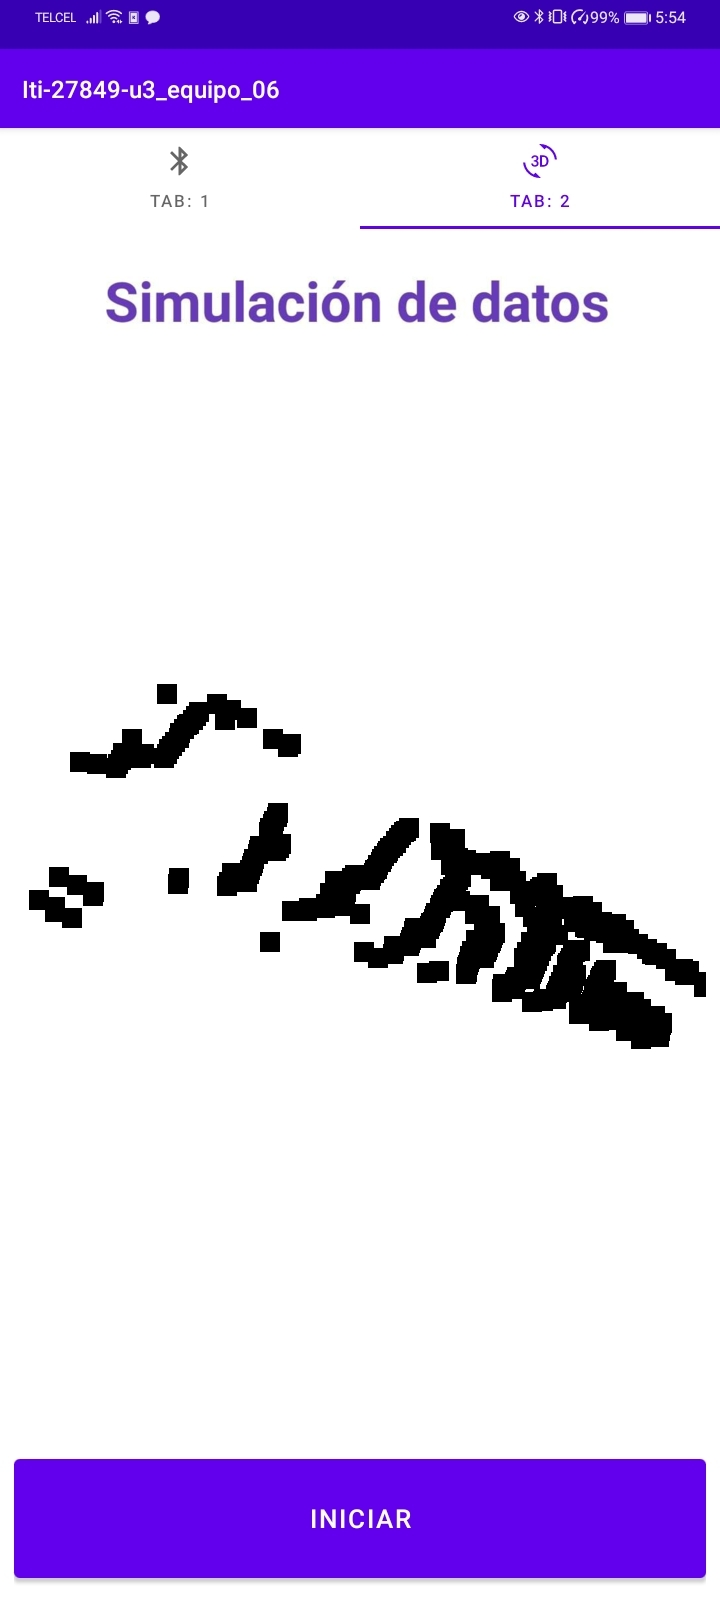
\includegraphics[width=0.14\textwidth]{2022_Scanner3D/figs/Ap2}
    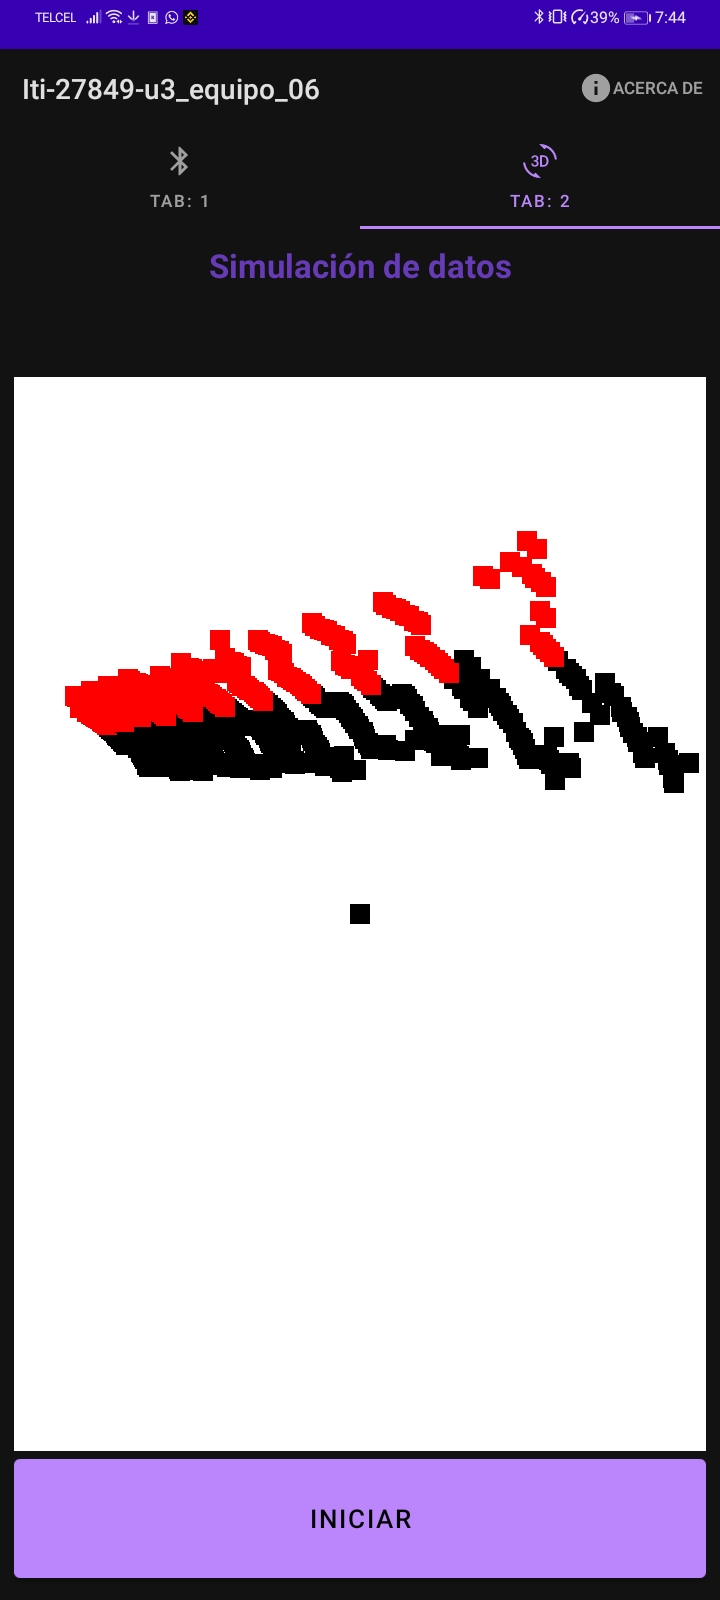
\includegraphics[width=0.14\textwidth]{2022_Scanner3D/figs/Ap3}
    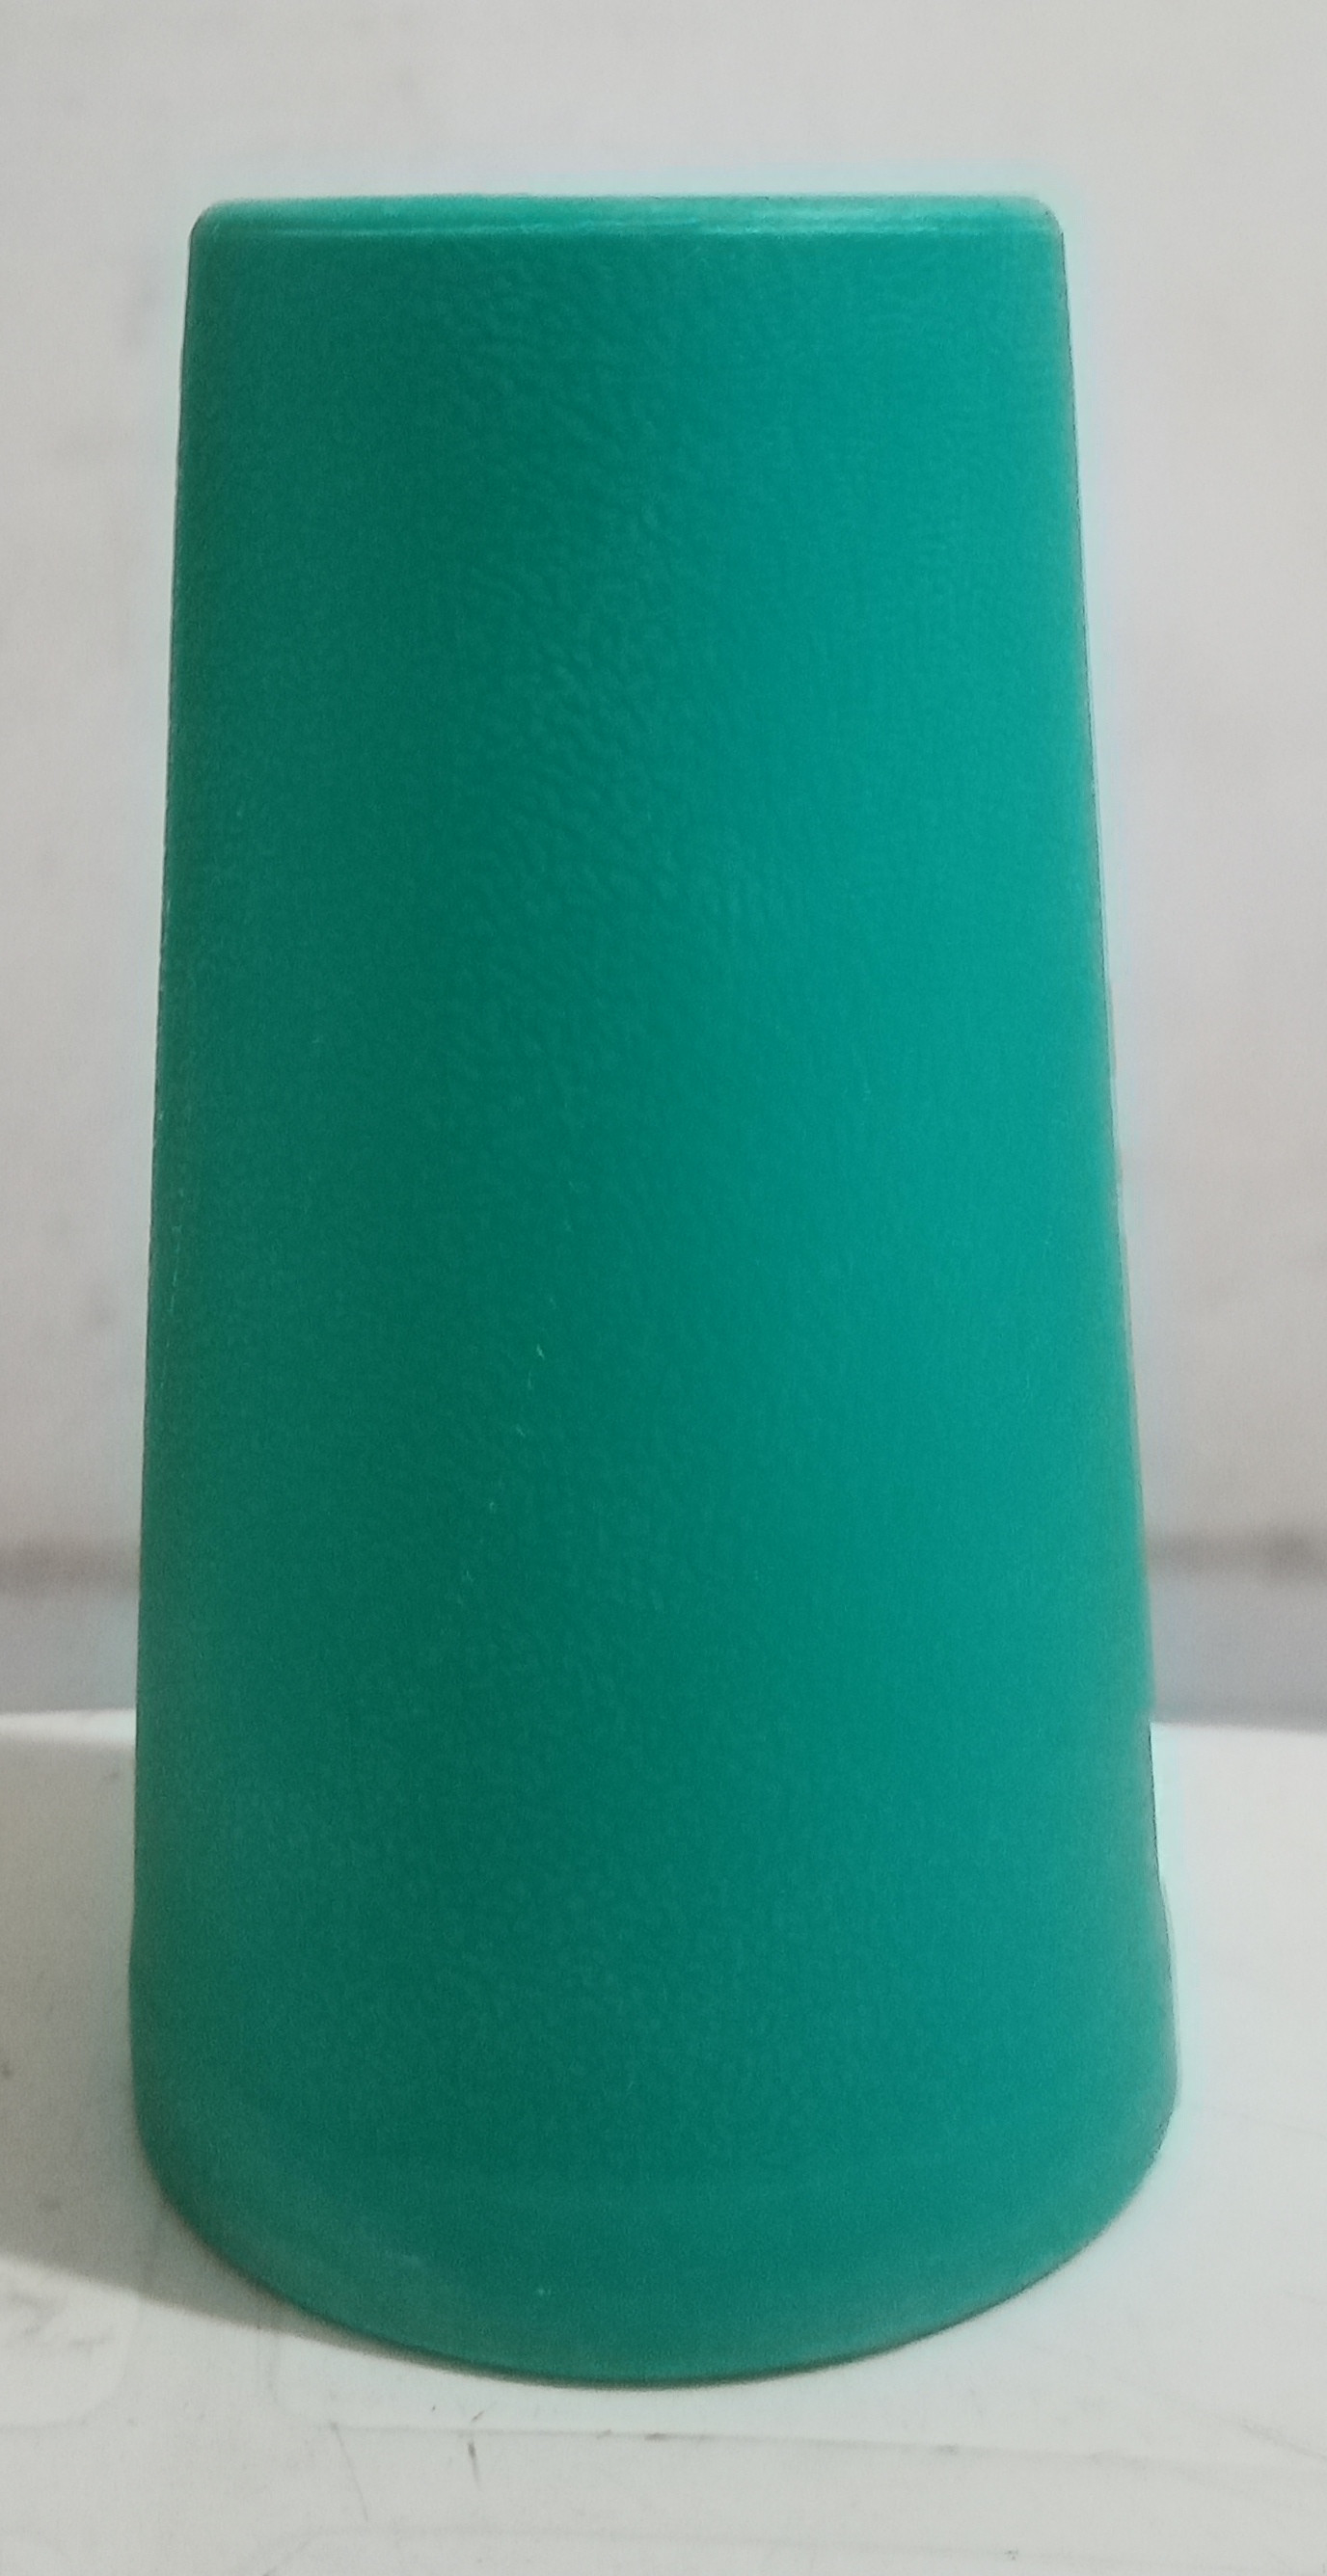
\includegraphics[width=0.16\textwidth]{2022_Scanner3D/figs/Ap4}
  \end{tabular}
\end{center}

\end{frame}






